\documentclass[conference]{IEEEtran}
\IEEEoverridecommandlockouts
\usepackage{cite}
\usepackage{amsmath,amssymb,amsfonts , nccmath}
\usepackage{algorithmic}
\usepackage{graphicx}
\usepackage{mathtools}

\usepackage{caption}
\usepackage{subcaption}
\usepackage{pgf-pie}  
\usepackage{textcomp}
\usepackage{xcolor}
\usepackage{multirow}
\usepackage{booktabs}
\usepackage{hyperref}



\newcommand\tab[1][1cm]{\hspace*{#1}}
\def\BibTeX{{\rm B\kern-.05em{\sc i\kern-.025em b}\kern-.08em
  T\kern-.1667em\lower.7ex\hbox{E}\kern-.125emX}}
   
  
   
\begin{document}

\title{Lung Tissue Classification using Graph Signal Processing in ILD patients}
\author{\IEEEauthorblockN{1\textsuperscript{st} Given Name Surname}
\IEEEauthorblockA{\textit{dept. name of organization (of Aff.)} \\
\textit{name of organization (of Aff.)}\\
Tehran, Iran \\
email address or ORCID}
\and
\IEEEauthorblockN{2\textsuperscript{nd} Given Name Surname}
\IEEEauthorblockA{\textit{dept. name of organization (of Aff.)} \\
\textit{name of organization (of Aff.)}\\
Tehran, Iran \\
email address or ORCID}
\and
\IEEEauthorblockN{3\textsuperscript{rd} Given Name Surname}
\IEEEauthorblockA{\textit{dept. name of organization (of Aff.)} \\
\textit{name of organization (of Aff.)}\\
Tehran, Iran \\
email address or ORCID}
\and
}

\maketitle

\begin{abstract}
\end{abstract}

\begin{IEEEkeywords}
ILD, Graph, Visibility graph, Textue classification
\end{IEEEkeywords}

\section{\large{Introduction}}
The interstitial lung disease (ILD), also referred ad the diffuse parenchymal lung disease, is a diverse group of lung diseases that incorporates over 150 various diseases due to similar clinical symptoms and radiographic results \cite{ILD_intro1}. ILD causes scarring (fibrosis) of the lung tissue, which eventually leads to difficulty breathing and absorbing enough oxygen through the lungs for the patient \cite{ILD_intro2}. Despite the clinical similarity between different types of ILDs, their mechanisms and treatment of them are varied from each other, and this fact greatens the importance of precise diagnosis\cite{dataset}. Through the years, high-resolution computed tomography (HRCT) images, alongside the clinical history of the patients, have become the gold standard for diagnosis of the ILD \cite{dataset}. Texture understanding plays an undeniable role in human understanding of images, and it is essential to efficient biomedical tissue description \cite{ILD_intro3}. As a result, computer-aided diagnosis (CAD) with the aim of texture classification became an active research field in past years to provide a second opinion about the type of disease alongside the practitioners to reduce the errors \cite{ILD_intro4}.

In this work, we are using a dataset that is collected at the University Hospitals of Geneva (HUG) \cite{dataset} consists of HRCT images of 125 patients with various ILD type diseases to evaluate our method of classification of the five most frequent ILD lung tissue categories which are Healthy (H), Emphysema (E), ground glass (GG), fibrosis (F) and micronodules (M). Figure \ref{fig:texture_example} shows an example for each lung tissue category.

\begin{figure}[tbh]
  \centering
  \begin{subfigure}{0.092\textwidth}
    \centering
    
\includegraphics[width=\linewidth]{images/micronodules.png}
    \caption{M}
  \end{subfigure}
  \centering
  \begin{subfigure}{0.092\textwidth}
    \centering
    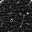
\includegraphics[width=\linewidth]{images/healthy.png}
    \caption{H}
  \end{subfigure}
  \centering
  \begin{subfigure}{0.092\textwidth}
    \centering
    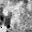
\includegraphics[width=\linewidth]{images/ground_glass.png}
    \caption{GG}
  \end{subfigure}
  \centering
  \begin{subfigure}{0.092\textwidth}
    \centering
    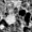
\includegraphics[width=\linewidth]{images/fibrosis.png}
    \caption{F}
  \end{subfigure}
  \centering
  \begin{subfigure}{0.092\textwidth}
    \centering
    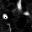
\includegraphics[width=\linewidth]{images/emphysema.png}
    \caption{E}
  \end{subfigure}
 
  \caption{An example for each lung tissue category}
  \label{fig:texture_example}
\end{figure}



%\subsection{\textbf{Related work:}}
The texture of more generally image classification can be performed with the deep learning methods or without them; without deep learning, we have two steps. First, we must develop and choose a feature extraction method and then train a classifier (e.g., SVM). On the other hand, the network learns the features with the deep learning method, and we do not need to extract them. 


Previous work in the literature that has been done on this dataset can be divided into using deep learning methods or not.
Guo et al. \cite{Fscore984} proposed a new version of DenseNet (SK-DenseNet) wich reaches the best F1-score of 98.4\% in the literature. Also Doddavarapu et al. \cite{acc9467} and Gao et al.\cite{acc928} used convolutional neural networks (CNN) to obtain the overall accuracy of 94.67\% and 92.8\% respectfully. Other not included deep learning methods used various feature extracting methods: gray-level co-occurrence matrices (GLCM) \cite{acc934},\cite{GLCM2} ,Grey level run length matrix (GLRLM)\cite{acc934}, histogram of Local Binary Patterns (LBP)\cite{acc934}, Large Margin Local Estimate(LMLE)\cite{acc861}, content–based image retrieval (CBIR) \cite{acc86} and local spectral analysis using a DCT-based filter bank \cite{Fscore89}.


As far as our knowledge, there is no previous work done with the graph signal processing (i.e., GSP) approach on the HUG dataset. Iacovacci et al. \cite{IVG} proposed a new way to define graphs for images and showed excellent performance on various tasks like texture classification. We used this method with slightly modification alongside the method proposed in \cite{wavelet} to achieve the overall accuracy of 97.05\% and an overall F1-score of 96.93\% which are the best results among non-deep learning methods and the second-best F1-score in deep learning methods with only 1.5\% difference with the best result. This study shows the excellent potential of the GSP methods for defining features for images that can be used in various other tasks.


\section{\large{Method}}
\subsection{\textbf{Graph wavelet filter banks}}

Wavelet filter banks are among the most popular methods for extracting features from images or textures. One of their variations is graph wavelet filter banks that consider the relation of different pixels in the texture. In this work, we used the method proposed by Qiao et al. at \cite{wavelet}. We used two-level decomposition for graph wavelet filters; after calculating the filter response with Meyer kernel on the texture as discussed in \cite{wavelet}, we moved a $4\times4$ window with the stride of 1 on the response of wavelet. For each window, we applied singular value decomposition. $F_1 , F_2, F_3$ sets as discussed in \cite{wavelet} are

\begin{equation}
\begin{multlined}
F_1=\{ max(S_1),max(S_2),...,\\max(S_i),...,max(S_N)\}\\
F_2=\{ mean(S_1),mean(S_2),...,\\mean(S_i),...,mean(S_N)\}\\
F_3=\{ median(S_1),median(S_2),...,\\median(S_i),...,median(S_N)\}
\end{multlined}
\end{equation}

After fitting a Weibull distribution to each set, we will get two parameters, scale and shape parameters.

For each texture, we have two level graph wavelets, and every wavelet has four subbands, every subband results in three $F_i$ sets, which will result in two parameters for Weibull distribution. Finally, we have a 48-dimensional feature vector for each texture.


Figure \ref{fig:weibull_fit} shows an example of weibull distribution fitting to $F_1$ and $F_2$ sets.
\begin{figure}[tbh]
  \centering
  \begin{subfigure}{0.24\textwidth}
    \centering
    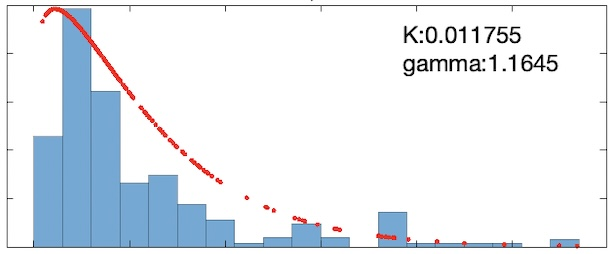
\includegraphics[width=\linewidth]{images/weibull1.jpg}
    \caption{}
  \end{subfigure}
  \hfill
  \begin{subfigure}{0.24\textwidth}
    \centering
    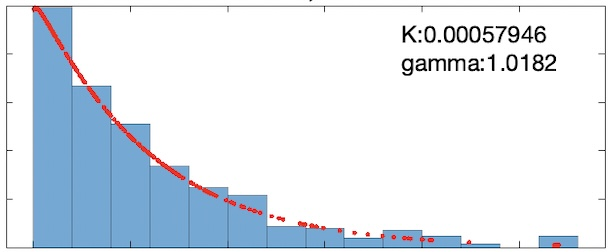
\includegraphics[width=\linewidth]{images/weibull2.jpg}
    \caption{}
  \end{subfigure}
  \caption{Example of Weibull fitting to $F_i$ sets}
  \label{fig:weibull_fit}
\end{figure}



\subsection{\textbf{Visibility Graphs}}
In recent yeast, increasing the popularity of complex systems and networks motivates researchers to develop methods for transforming classic signals into graph signals which help indicate the relation of signal values. one of these methods is called visibility graphs which are introduced in \cite{VG}. This method proposed in that paper is mainly applied to 1D signals. However, the concept is the same for higher dimension signals. As we know, images are 2D signals, and Iacovacci et al. in \cite{IVG} proposed a new version of visibility graphs for images called image visibility graphs.



\subsubsection{Natural Visibility Graphs}
We can connect the visibility line between two nodes with any slope in this definition. Instead, we can only have horizontal visibility lines in the horizontal visibility graph.
for the time series signal $S(t)=\{x_1,x_2,x_3,...,x_N\}$, we can define a N node natural visibility graph (N is the numbet of signal points) which $x_i$ and $x_j$ are connected only if we can find a line from $x_i$ to $x_j$ without intercepting other signal values.Equivalently $x_i$ and $x_j$ are connected if following constraint is hold,
\begin{equation}
x_k < x_i +\frac{k-i}{j-i}(x_j-x_i), \forall(i<k<j)
\end{equation}



\subsubsection{Horizontal Visibility Graphs}
The definition of horizontal visibility graphs is the same as natural visibility graphs, but we are only allowed to have horizontal lines instead of any slope for visibility lines. The Following equation depicts this definition,
\begin{equation}
x_k < inf(x_i, x_j), \forall(i<k<j)
\end{equation}

Figure \ref{fig:VG_example} is an example of HVG and NVG for a time-series signal.


\begin{figure}[tbh]
  \centering
  \begin{subfigure}{0.5\textwidth}
    \centering
    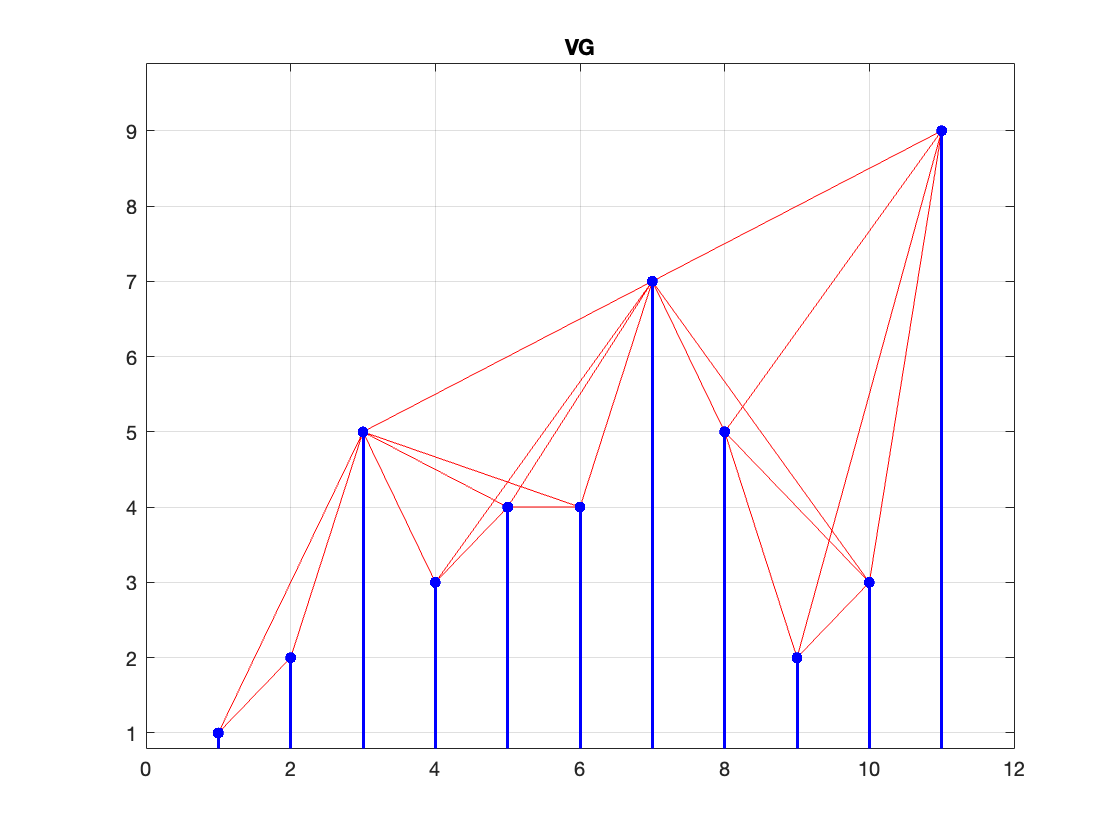
\includegraphics[width=\linewidth]{images/VG.png}
    \caption{Natural visibility graph}
    \label{fig:NVG_example}
  \end{subfigure}
  \hfill
  \begin{subfigure}{0.5\textwidth}
    \centering
    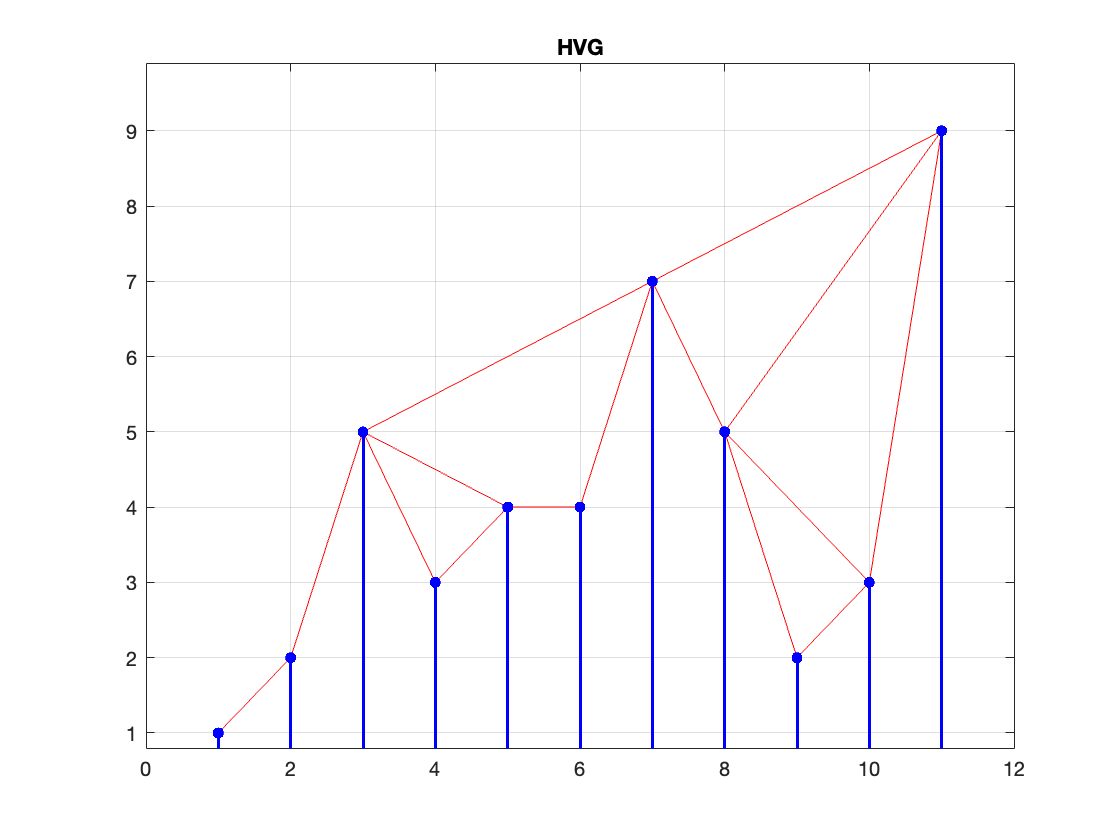
\includegraphics[width=\linewidth]{images/HVG.png}
    \caption{Horizontal visibility graph}
    \label{fig:HVG_example}
  \end{subfigure}
  \caption{Example of NVG and HVG for a time series signal}
  \label{fig:VG_example}
\end{figure}



\subsection{\textbf{Image Visibility Graphs}}
Visibility graphs showed a great potential to define the relation in time series signals, and they easily apply to 2D signals, i.e., images. Iacovacci et al. at \cite{IVG} developed the idea of visibility graphs for images. We had two definitions in time series signals for VG's, and we also have two definitions for image visibility graphs derived from the time series version of VG's.

\subsubsection{\textbf{INVG} (Image natural visibility graph)}
The natural visibility graph for an $N\times N$ image is a graph with $N^2$ nodes. Each node corresponds to a pixel, and the node's value is equal to the intensity of the corresponding image pixel. Each node is labeled as $I_{ij}$ wich $i$ and $j$ indicate the position of the pixel in the image.

According the definition proposed in \cite{IVG},nodes $I_{ij}$ and node $I'_{i'j'}$ are connected if following conditions hold,

\vspace{0.5cm}
\begin{itemize}
\setlength{\itemindent}{.5cm}
\item \emph{$(i=i')$ $OR$ $(j=j')$ $OR$ \\
\tab $ [\exists k \in \mathbb{Z} : \big((i=i'+k)\, AND \, (j=j'+k)\big)]$} 
\vspace{0.1cm}
\item \emph{$I_{ij}$ and $I'_{i'j'}$ are connected in the sequence \tab $\big\{I_{ij},I'_{i'j'},ij, i'j'\big\}$ 
 with the definition of NVG for \tab time-series signals.}
\end{itemize}
\vspace{0.5cm}



\subsubsection{\textbf{IHVG} (Image Horizontal visibility graph)}
The definition of the IHVG is the same as the INVG, but in the second condition, we have to change NVG with the HVG.

\subsubsection{\textbf{Global and local features for IVG's}}
After defining the IVGs, we have to extract features to use them for classification; Iacovacci et al. at \cite{IVG} introduced global features to comprise global properties of the image and local features for compacting the local characteristics of the image. For the global feature, we used degree distribution, $p(k)$, and visibility patch with the order of 3, $VP_3$ as defined in \cite{IVG} for the local feature, even though the global feature did not use in the final feature selection process which is discussed in section \ref{feature_selecting}



\section{\large{Feature selection}}\label{feature_selecting}
This section will discuss the various features that we can choose for our final feature vector; firstly, we discuss each component individually and then demonstrate the final feature vector.


\subsubsection{\textbf{Image, reversed-image}}
As we showed before, the nature of the IVG and HVG definition behaves differently about the local maxima, so taking into account this fact, we calculate features for the original image and reverse image, which is obtained by replacing each pixel value with the maximum pixels value subtracted by the current pixel value.
Figure \ref{fig:original_reversed_texture} shows an example of a texture and its reverse.

\begin{figure}[tbh]
  \centering
  \begin{subfigure}{0.24\textwidth}
    \centering
    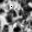
\includegraphics[width=0.55\linewidth]{images/origianl_fibrosis.png}
    \caption{Original image}
    \label{fig:original_texture}
  \end{subfigure}
  \hfill
  \begin{subfigure}{0.24\textwidth}
    \centering
    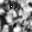
\includegraphics[width=0.55\linewidth]{images/reversed_fibrosis.png}
    \caption{Reversed image}
    \label{fig:reversed_texture}
  \end{subfigure}
  \caption{original and reversed image of a Fibrosis texture}
  \label{fig:original_reversed_texture}
\end{figure}



\subsubsection{\textbf{IHVG, INVG}}
As we discussed before, we had to choose to define our graphs on images,i.e., natural or horizontal visibility graphs. Our investigation indicates that both of these definitions are useful for describing the textures, and we finally chose features from both of these graph types.
Figure \ref{fig:lattice_nolattice_example} is an artifial $3\times3$ image and INVG is drawn for with Lattice and with No-lattice condition.



\begin{figure}[tbh]
  \centering
  \begin{subfigure}{0.24\textwidth}
    \centering
    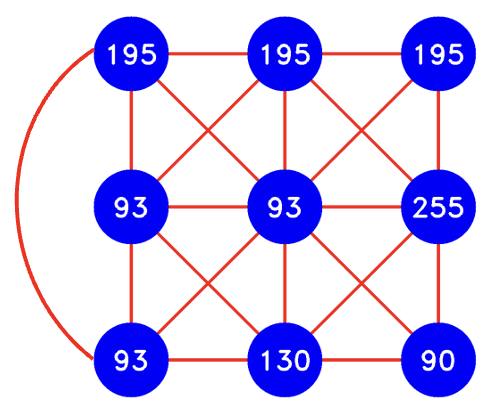
\includegraphics[width=0.55\linewidth]{images/Lattice_IVG.png}
    \caption{With lattice}
    \label{fig:lattice_example}
  \end{subfigure}
  \hfill
  \begin{subfigure}{0.24\textwidth}
    \centering
    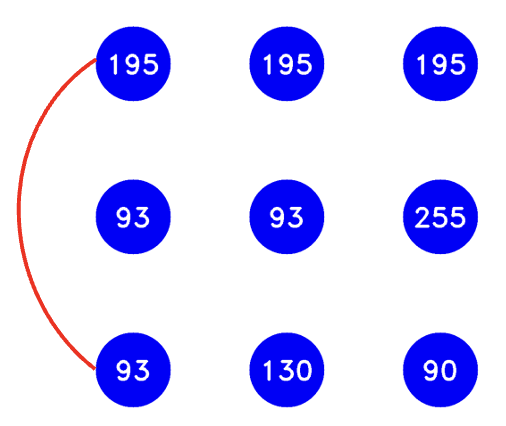
\includegraphics[width=0.55\linewidth]{images/Nolattice_IVG.png}
    \caption{Without lattice}
    \label{fig:nolattice_example}
  \end{subfigure}
  \caption{An example of INVG with and without lattice}
  \label{fig:lattice_nolattice_example}
\end{figure}


\subsubsection{\textbf{Lattice, without lattice}}
Based on the definition of a visibility graph, each pixel is connected to all of the neighbor pixels, so for simplicity, we can choose to consider these links or not. If we decided not to consider these links, we would have a visibility graph with no-lattice and vice versa. No-lattice graphs result in a more simple graph representation and a more sparse adjacency matrix.


It is good to mention that we can choose both local and global features for each visibility graph configuration; we implemented local feature extraction with $3\times3$ windows and stride one. Also, for global features, we calculate the degree distribution for the graph and plot the histogram of it, then fit a Weibull distribution to that, which will give us two elements for the feature vector, so each of the visibility graph feature vectors is a 258-dimensional vector which the first 256 element is for local feature extraction, and the rest is for global features.

\subsubsection{\textbf{wavelet}}
The method discussed in \cite{wavelet} is a very innovative approach to defining a graph-based feature vector for a texture. We implement that method with a 2-level bipartite graph, and two levels of image,i.e., only one subsampling from $32\times32$ texture resulting in a $16\times16$ texture, and with Meyer kernel for graph wavelet filter with a filter length of 24.
This method for each texture results in a 48-dimensional feature vector, and we can calculate it for both original textures and reversed textures, as discussed before. 


\subsubsection*{\textbf{Final choice}}
Suppose we concatenate all of the possible choices for the final feature vector. In that case, it will give us a 2160-dimensional feature vector for a $32\times32$ texture image which is not desired and can cause overfitting of the model and harder convergence for the classifier. So we sort each feature vector component based on their part in the total variance of data; this job is done by the same strategy of primary component analysis. Before that, we have to make the feature vectors zero-mean and unit length (due to zero-mean, this has the same effect of making the data unit variance) to make all data have the same scale. Otherwise, we do not get the correct result. Also, an essential consideration in machine learning theory is to only perform PCA and data-preprocess (zero-mean and unit length) on Train data, which will be discussed later and not on the full dataset.
Figure \ref{fig: PCA1} shows a pie chart that indicates part of the total variance of data for each possible feature vector component. We should mention that sum of the variance of all global feature extraction methods for visibility graph components was only 1.3\% of all variance. Hence, we decided to remove them from the final feature vector for training our classifier. We concatenate all possible feature vector components except three\: Image-IVG-Nolattice, Reversed-Image-HVG-Nolattice, and Reversed-Image-IVG-Nolattice, which will give us a 1376-dimensional feature vector for each texture.

\begin{figure}[tbh]
 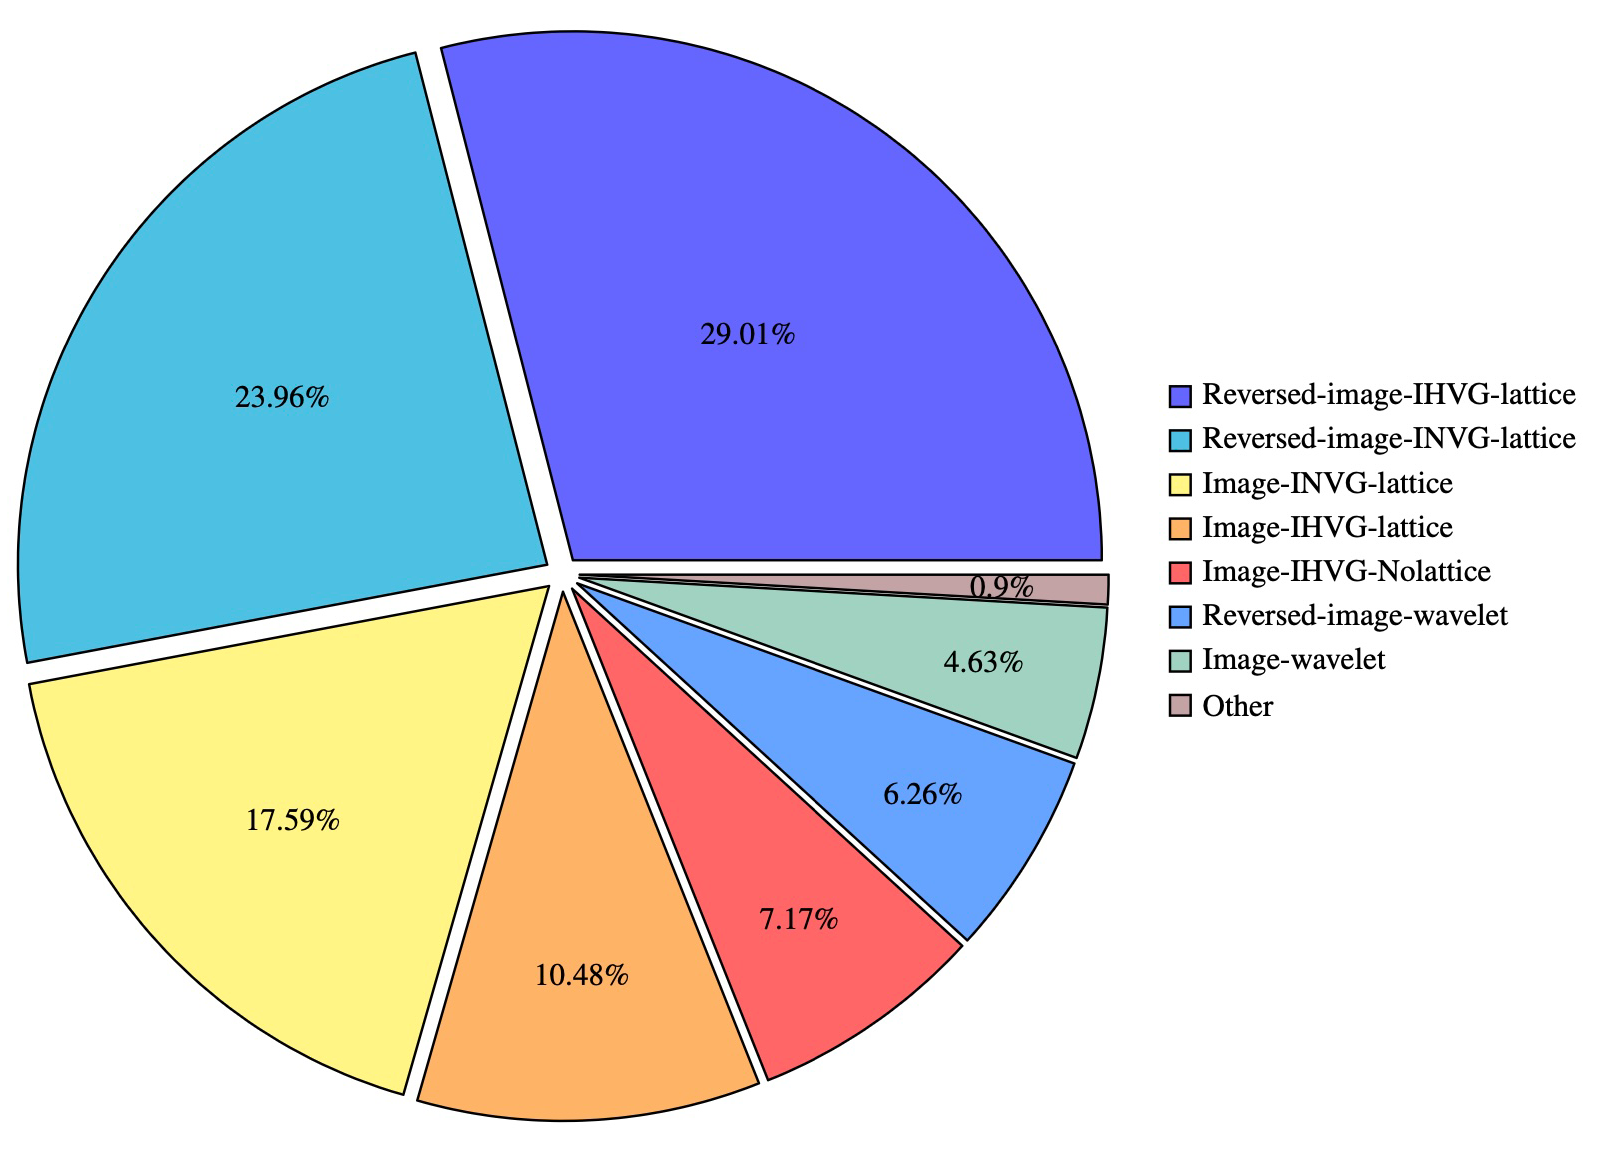
\includegraphics[width=1\linewidth]{images/PCA_piechart.png}
   \caption{Importance of each feature vector component based on the variance of all data}
 \label{fig: PCA1}
\end{figure}


\section{\large{Experiments and results}}
\subsection{\textbf{Dataset}}
We used a dataset of interstitial lung disease (ILD) \cite{dataset} cases containing HRCT images of 128 patients with the inter-slide distance of 10mm, slice thickness of 1mm, and in-plane resolution of $512\times 512$ pixels. In each 2D-single image of a patient, regions of interest (ROIs) are hand-drawn and labeled by two expert radiologists with 20 and 15 years of experience used as ground truth. 

The dataset consists of 17 types of lung textures, but in this work, we only used the five most frequent ones, which are Healthy (H), Ground glass (GG), Micronodules (M), Emphysema (E), and Fibrosis (F). This choice only left us 108 patients from a total patient number of 128.

For detecting and extracting textures from HRCT image series, in each 2D image with defined ROIs, we moved a window with the size of $32 \times 32 $ pixels on the lung mask and if the percentage of window area that covers the specific ROI with a defined texture label was greater than a chosen threshold (the chosen threshold is 0.8).


For extracting textures, we mainly used the implementation that Anthimopoulos et al. \cite{textureextract} provided in a GitHub repository \footnote{ \url{https://github.com/ChelovekHe/ild-cnn}}. However, we modified and adjusted the code for our work.

Table \ref{cm:datadist} shows the distribution of textures among various classes.



\begin{table}[tbh]
 \caption{\small{Distribution of patches among different tissue categories}}
\label{cm:datadist}
\small
\centering
\begin{tabular}{@{}llllll@{}}
\toprule
 Tissue Category& \# patients & \# patches & \\ \midrule
 
H& 15&7828 \\ 
GG&33&2986\\ 
M&18 &11629 \\ 
E&9 &1981 \\ 
F& 39&5251 \\ \bottomrule

\end{tabular}
\end{table}



\subsection{\textbf{Data preprocessing \& Classifier}}
Due to unbalanced data distribution between various classes, we used five-fold stratified cross-validation. For each fold, we make train data zero-mean with a unit length. Then, with the aim of the primary component analysis, we only chose features that makeup 94.85\% of all data variation. Before PCA feature vector length was 1376, and after PCA was 616. We must use the same transform applied to train data for data to preprocess and PCA for test data in each fold. After this transformation, the mean of the test data is not necessarily zero.

For the classifier, we used support vector machine, SVM, with a gaussian kernel and one-vs-other strategy for our multiple class problem. Also, to address the imbalanced distribution of data between classes, we used weighted SVM to solve this issue,i.e., for the class with the least data, the SVM weight is the largest.





\subsection{\textbf{Performance evaluation}}
After extracting features and preprocessing the data, all data are randomly partitioned into five parts. One of the parts is used for test data and the others for train. This process is repeated five times, and each time a different partition is used for test data, so in the end, all of the data is used for testing. This method is called five-fold cross-validation. After training an SVM classifier in each fold, we concatenate the result for the test partition, and a final evaluation is performed on this concatenated set. The following metrics measure our method's performance, and for each class, we used the one-vs-rest (i.e., OVR) policy.


\small \begin{equation}
Accuracy = \frac{TP\,+\,TN}{TP\,+\,TN\,+\,FP\,+\,FN} \nonumber
\end{equation}
\small \begin{equation}
Recall = \frac{TP}{TP\,+\,FN} \nonumber
\end{equation}
\small \begin{equation}
Precision = \frac{TP}{TP\,+\,FP} \nonumber
\end{equation}
\small \begin{equation}
TN-rate = \frac{TN}{TN\,+\,FP} \nonumber
\end{equation}
\small \begin{equation}
F1-score = \frac{2TP}{2TP\,+\,FP\,+\,FN}\nonumber
\end{equation}
\small \begin{equation}
AUC = the\,area\,under\, the\, ROC\, curve  \nonumber
\end{equation}

Table \ref{cm:CM} shows the confusion matrix for the final classifier. In table \ref{cm:result}, we summarize the performance of our method for each class and also overall classification performance.



\begin{table}[tbh]
\caption{Confusion Matrix for texture classification}
\label{cm:CM}
\small
\centering
\begin{tabular}{@{}lllllllll@{}}
&& \multicolumn{3}{c}{Predicted label}\\
\toprule
 & H & GG & M & E & F \\ \midrule
 
H& 7688 & 51 & 73 & 11 & 5 \\ 
GG& 80 & 2851 & 21 & 0 & 34 \\ 
M& 286 & 43 & 11214 & 4 & 82 \\ 
E& 42 & 6 & 11 & 1917 & 5 \\ 
F& 20 & 57 & 42 & 3 & 5129 \\ \bottomrule

\end{tabular}
\end{table}




\begin{table}[tbh]
\caption{Results}
\label{cm:result}
\centering
\begin{tabular}{@{}lllllllll@{}}
\toprule
\multirow{0}{0.5cm}{} & \multirow{1}{0.8cm}{\centering{{Accuracy}}} & \multirow{1}{0.8cm}{Recall}&\multirow{1}{0.8cm}{Precision} & \multirow{1}{1cm}{TN-rate} & \multirow{1}{0.8cm}{AUC} & \multirow{1}{1cm}{F1-score} \\ \midrule

H & 98.09\% & 98.21\% & 94.73\% & 98.04\% & 98.13\% & 96.44\% \\ 
GG & 99.02\% & 95.48\% & 94.78\% & 99.41\% & 97.45\% & 95.13\% \\ 
M & 98.11\% & 96.43\% & 98.71\% & 99.19\% & 97.81\% & 97.56\% \\ 
E & 99.72\% & 96.77\% & 99.07\% & 99.94\% & 98.35\% & 97.91\% \\ 
F & 99.16\% & 97.68\% & 97.6\% & 99.48\% & 98.58\% & 97.64\% \\  \bottomrule
\vspace{-0.25cm} \\ 
Overal & 97.05\% & 96.98\% & 96.91\% & 99.21\% & - & 96.93\% \\ 
\vspace{-0.3cm} \\ 
\bottomrule

\end{tabular}
\end{table}


\subsection{\textbf{Comparison to previous work}}
In this subsection, we compare our result with some of the recent performances on the ILD texture classification; table \ref{cm:compare} shows this comparison.



\begin{table}[tbh]
  \caption{\centering{\small{Comparison of ILD texture classification with the state-of-the-art performances.}}}
  \label{cm:compare}
  \centering
  \scriptsize
  \begin{tabular}{@{}lllllllll@{}}
  \toprule
  \multirow{1}{0.8cm}{\textbf{Reference}} & \multirow{1}{0.7cm}{\centering{\textbf{Accuracy}}} & \multirow{1}{0.9cm}{\textbf{F1-score}} & \multirow{1}{2cm}{{\textbf{Method}}} \\ \midrule

Dudhane et al. \cite{acc934} & 93.41\% & - & GLCM, GLRLM, hist. of LBP\\ 
Song et al. \cite{acc861} & 86.1\% & - & LMLE \\ 
Depeursinge et al. \cite{acc86} & 86\% & - & CBIR, 3D localization\\ 
Doddavarapu et al. \cite{acc9467} & 94.67\% & - & CNN model\\ 
Gao et al.\cite{acc928} & 92.8\% & - & CNN model\\  
Anthimopoulos et al. \cite{Fscore89} & - & 89\% & DCT filter bank,gray-level hist.\\  
Guo et al. \cite{Fscore984} & - & 98.4\% & SK-DenseNet (CNN model)\\  
Huang et al. \cite{Fscore96} & - & 96\% & CNN model \\  \bottomrule

  \vspace{-0.23cm} \\ 
  \textbf{Our method} & \textbf{97.05\%} & \textbf{96.93\%} & \textbf{IVG, graph wavelet }\\ 
  \vspace{-0.3cm} \\ 
  \bottomrule
   
\end{tabular}
\end{table}



\section{\large{Conclusions}}
Our study evaluated the performance of graph signal processing (i.e., GSP) methods to classify the five most frequently appeared lung tissues in ILD patients. Some of the previous works that have been done in the literature are only using the deep learning method for feature extraction. Generally, they get higher accuracy on this dataset. Although we insist on not using the deep learning method, we achieved higher performances than most of these methods and the best performance in the classic methods. We inspired our work by the success of \cite{chinaIVG}, and \cite{wavelet} using the image visibility graphs and graph wavelets for texture classification.

The nature of the visibility graph differentiates between local minima and maxima in the signal, so we calculated the IVG for both the original and reverse image. This action improved the overall accuracy by almost five percent.

As far as our knowledge, we performed the first graph-based techniques for classifications of ILD tissues. Compared to others, our result on this complex dataset indicates the high potential of GSP for various tasks like texture classification.



\bibliographystyle{IEEEtran}
\bibliography{allref.bib}
\vspace{12pt}
\end{document}




